\documentclass[12pt]{article}

% Packages
\usepackage{amsmath, amssymb, amsthm}
\usepackage{geometry}
\usepackage{fancyhdr}
\usepackage{enumitem}
\usepackage{titlesec}
\usepackage{caption}
\usepackage{tcolorbox}
\usepackage{float}

% Page Setup
\geometry{margin=1in}
\setlength{\parindent}{0pt}
% \setlength{\parskip}{0em}
\setcounter{secnumdepth}{3}

\pagestyle{fancy}
\fancyhf{}
\lhead{Ethan Fan}
\rhead{PCH}
\cfoot{\thepage}

\allowdisplaybreaks

% Section Formatting
\titleformat{\section}
  {\bfseries}
  {}
  {0em}
  {}
\titlespacing*{\section}{0pt}{0pt}{0.3em}

\titleformat{\subsection}[runin]
  {\bfseries}
  {}
  {0em}
  {}
\titlespacing*{\subsection}{0pt}{0pt}{0em}

\titleformat{\subsubsection}[runin]
  {\itshape}
  {(\roman{subsubsection})}
  {0em}
  {}

% mathematical commands
\newcommand{\ddt}{\frac{d}{dt}}
\newcommand{\ddx}{\frac{d}{dx}}
\newcommand{\dydx}{\frac{dy}{dx}}
\newcommand{\tor}{\text{ or }}
\newcommand{\dne}{\ \mathrm{DNE}}
\newcommand{\floor}[1]{\lfloor #1 \rfloor}

\newcommand{\sub}[1]{\subsection{(#1)} \,}

\newcommand{\definition}[1]{\begin{tcolorbox}[colback=red!5!white,colframe=red!75!black,parbox=false] #1 \end{tcolorbox}}

\newcommand{\theorem}[2]{\begin{tcolorbox}[title={#1},colback=blue!5!white,colframe=blue!75!black,parbox=false] #2 \end{tcolorbox}}

\newcommand{\example}[2]{\begin{tcolorbox}[title={Example: #1},colback=brown!5!white,colframe=brown!75!black,parbox=false] #2 \end{tcolorbox}}

\newcommand{\remark}[2]{\begin{tcolorbox}[title={#1},colback=black!5!white,colframe=black!75!black,parbox=false] #2 \end{tcolorbox}}

% Document
\begin{document}

\vspace*{0cm}

\begin{center}
    {\Large \bfseries Problem Set 61} \\[0.5cm]
    {\large Continuity 2} \\[0.35cm]
    {\normalsize April 3, 2026}
\end{center}

% Questions

\theorem{The Intermediate Value Theorem (IVT)}{Suppose that $f(x)$ is continuous on a closed interval $[a,b]$ and let $N$ be any number between $f(a)$ and $f(b)$, where $f(a) \ne f(b)$. Then, there exists a number $c \in (a,b)$ such that $f(c)=N$.}

\section{Example 1}
$f(x)=x^3-3x-19 $ or $ x^3-3x-19=0$ on interval $[1,5] \implies a=1,b=5$ \vspace{0.3em} \\
1. $f(x)$ is a continuous polynomial function on $[1,5]$.\\
2. $f(1)=-21, f(5)=91$
\[
-21<N<91 \implies \text{let }N=0
\]
3. By the Intermediate Value Theorem, since $f(x)$ is continuous on $[1,5]$, and $f(1)<0<f(5)$, then there exist a number $c\in (1,5)$ such that $f(c)=0$. i.e. $c^3-3c-19=0$ is solvable on $(1,5)$. \vspace{0.5em}

\section{Question 3}
Sketch the graph of $f(x)=\floor{\sin x + \cos x}, \ x \in [0,2\pi]$ and discuss its continuity.
\begin{gather*}
    f(x)=\floor{\sin x + \cos x}=\floor{\sqrt{2}\sin(x+\arctan \frac{1}{1})}=\floor{\sqrt{2}\sin (x+\frac{\pi}{4})}\\
    R_{f(x)}=\begin{cases}
        1 \quad &x \in [0, \frac{\pi}{2}] \cup \{2\pi\}\\
        0 \quad &x \in (\frac{\pi}{2}, \frac{3\pi}{4}] \cup [\frac{7\pi}{4}, 2\pi)\\
        -1 \quad &x \in (\frac{3\pi}{4}, \pi] \cup [\frac{3\pi}{2}, \frac{7\pi}{4})\\
        -2 \quad &x \in (\pi, \frac{3\pi}{2})
    \end{cases}
\end{gather*}

\begin{figure}[H]
    \centering
    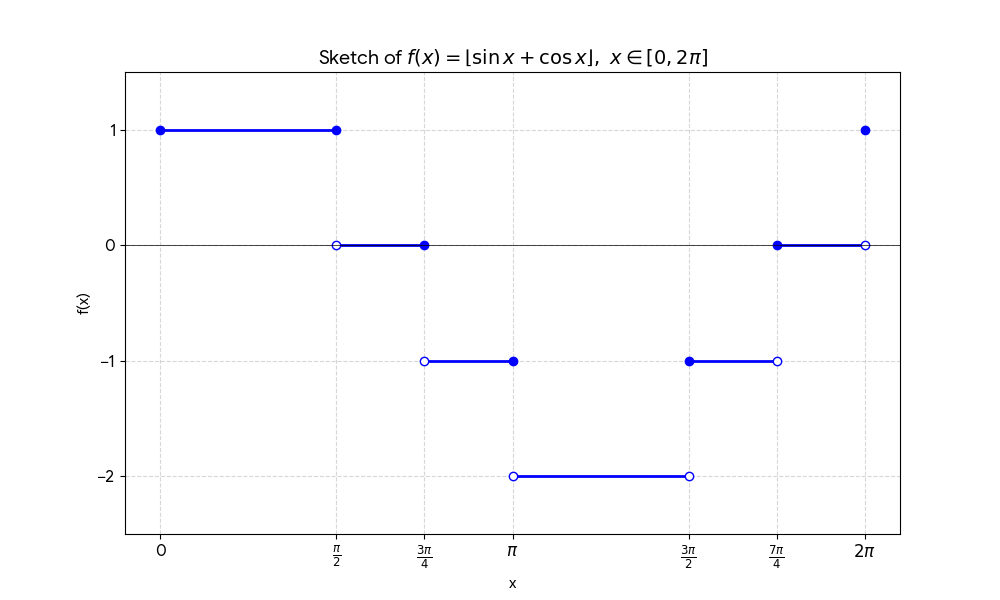
\includegraphics[width=0.6\linewidth]{sincos.png}
    \label{fig:placeholder}
\end{figure}

\begin{gather*}
    \lim_{x\to \frac{\pi}{2}^-}f(x)= \lim_{x\to \frac{\pi}{2}^-} \floor{\sqrt{2} \sin (x+\frac{\pi}{4})} = \lim_{x\to \frac{\pi}{2}^-} 1= 1\\
    \lim_{x\to \frac{\pi}{2}^+}f(x)= \lim_{x\to \frac{\pi}{2}^+} \floor{\sqrt{2} \sin (x+\frac{\pi}{4})} = \lim_{x\to \frac{\pi}{2}^+} 0= 0\\
    \lim_{x\to \frac{\pi}{2}^-}f(x) \ne \lim_{x\to \frac{\pi}{2}^+ }f(x) \implies \lim_{x\to \frac{\pi}{2}}f(x) \dne 
\end{gather*}
Similarly,
\begin{gather*}
    \lim_{x\to \frac{3\pi}{4}}f(x), \lim_{x\to \pi}f(x), \lim_{x\to \frac{3\pi}{2}}f(x), \lim_{x\to \frac{7\pi}{4}}f(x), \lim_{x\to 2\pi}f(x)  \dne \\
    \boxed{f(x) \text{ is continuous on } \{ x | x\in [0, 2\pi], \quad  x \notin \{\frac{\pi}{2}, \frac{3\pi}{4}, \pi, \frac{3\pi}{2}, \frac{7\pi}{4}, 2\pi \}}
\end{gather*}

\section{Question 4}
Discuss the continuity of $f(x) = |x| sgn (x^3-x)$
\begin{gather*}
    f(x) = |x| sgn (x^3-x) = |x|sgn (x(x+1)(x-1))\\
    f(x)=\begin{cases}
        x \quad &x \in ( -\infty , -1) \cup (1, \infty)\\
        0 \quad &x \in \{-1,0,1\}\\
        -x \quad & x \in (-1,0) \cup (0,1)
    \end{cases}\\
    \lim_{x \to -1^-} f(x) = \lim_{x \to -1^-} x = -1\\
    \lim_{x \to -1^+} f(x) = \lim_{x \to -1^+} -x = 1\\
    \lim_{x \to -1^-} f(x) \ne \lim_{x \to -1^+} f(x) \implies \lim_{x \to -1} f(x) \dne\\
    \lim_{x \to 1^-} f(x) = \lim_{x \to 1^-} -x = -1\\
    \lim_{x \to 1^+} f(x) = \lim_{x \to 1^+} x = 1\\
    \lim_{x \to 1^-} f(x) \ne \lim_{x \to 1^+} f(x) \implies \lim_{x \to 1} f(x) \dne\\
    \boxed{f(x) \text{ is continuous on } \{ x | x\in \mathbb{R}, \quad x \notin \{-1,1\}}
\end{gather*}

\section{Question 5}
Discuss the continuity of $f(x) = 1 + \lim\limits_{n \to \infty} \cos ^{2n} x$. Sketch the graph to support your answer.
\begin{gather*}
    f(x)=1+\lim\limits_{n \to \infty} \cos ^{2n} x =1+\lim_{n \to \infty} (\cos^2 x)^n\\
    \cos^2 x \in  \begin{cases}
        \{1\} \quad &x=k\pi, \quad k\in \mathbb{Z}\\
        [0,1)\quad &x\ne k\pi, \quad k\in \mathbb{Z}
    \end{cases}\\
    \lim_{x \to k\pi^-} f(x) = \lim_{x \to k\pi^-} (1+\lim\limits_{n \to \infty} \cos ^{2n} x) = 1+0=1\\
    \lim_{x \to k\pi^+} f(x) = \lim_{x \to k\pi^+} (1+\lim\limits_{n \to \infty} \cos ^{2n} x) = 1+0=1\\
    \lim_{x \to k\pi^-} f(x) = \lim_{x \to k\pi^+} f(x) \implies \lim_{x \to k\pi} f(x) = 1\\
    f(k\pi)=1+\lim_{n \to \infty}(\cos^2 x)^n=1+1^n=2\\
    \lim_{x \to k\pi} f(x) \ne f(k\pi)\\
    \boxed{f(x) \text{ is continuous on } \{ x | x\in \mathbb{R}, \quad x \ne k\pi, \quad k \in \mathbb{Z} \}}
\end{gather*}

\begin{figure}[H]
    \centering
    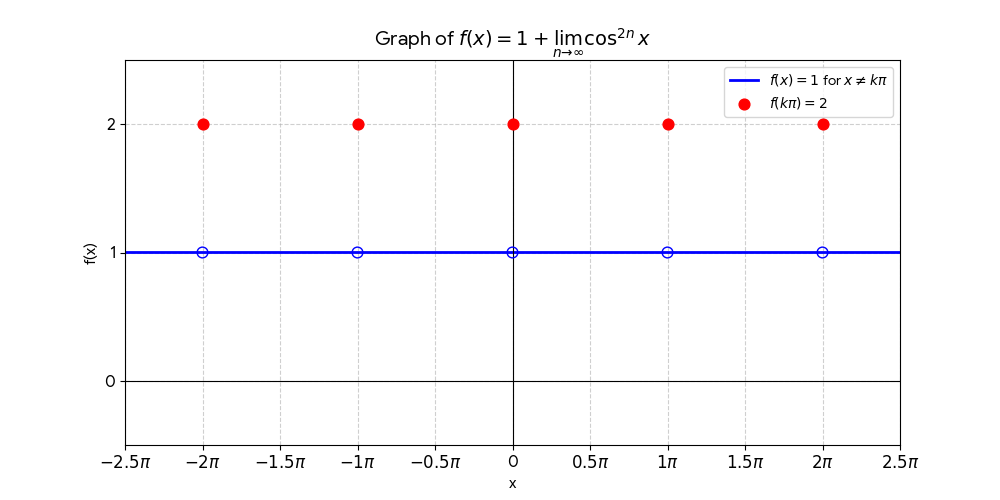
\includegraphics[width=0.6\linewidth]{limcos.png}
    \label{fig:placeholder}
\end{figure}

\section{Question 6}
Discuss the continuity of the function: $f(x)=\begin{cases}
    1 \quad \text{if $x$ is rational}\\
    0 \quad \text{if $x$ is irrational.}
\end{cases}$\vspace{0.3em} \\ 
Define $q$ and $i$ to be arbitrary values satisfying $q \in \mathbb{Q}$ and $i \in \mathbb{Q}^c$.
\begin{gather*}
    \lim_{x \to q^-} f(x) = f(q^-) \to 0 \tor 1 \implies \lim_{x\to q} f(x)\dne \\
    \lim_{x \to i^-} f(x) = f(i^-) \to 0 \tor 1 \implies \lim_{x\to i} f(x)\dne \\
    \boxed{\text{The Dirichlet function is discontinuous on $\mathbb{R}$}}
\end{gather*}

\section{Question 7}
Find the value of $x$ such that the function $f(x) = \begin{cases}
    x \quad &\text{if $x$ is rational}\\
    1-x \quad &\text{if $x$ is irrational}
\end{cases}$ is continuous. \vspace{0.3em} \\
\begin{gather*}
    \lim_{x \to a^-} f(x) = f(a^-) \to a \tor 1-a\\
    a=1-a \implies a=\frac{1}{2}\\
    \boxed{f(x) \text{ is continuous on } x=\frac{1}{2}}
\end{gather*}

\section{Question 10}
Use the Intermediate Value Theorem to prove that the function has at least one real root (intercept) in a given interval. Follow the format outlined in class. \vspace{0.3em}

\subsection{(a)} \, $f(x)=4x^3 - 6x^2+3x-2, \qquad [1,2]$\\
1. $f(x)$ is a continuous polynomial function on $[1,2]$.\\
2. $f(1)=-1, f(2)=12$
\[
-1<N<12 \implies \text{let }N=0
\]
3. By the Intermediate Value Theorem, since $f(x)$ is continuous on $[1,2]$, and $f(1)<0<f(2)$, then there exist a number $c\in (1,2)$ such that $f(c)=0$. i.e. $4x^3 - 6x^2+3x-2=0$ is solvable on $(1,2).$ \vspace{0.3em}

\subsection{(b)} \, $f(x)=x^3-4x+\cos \pi x, \qquad [0,1]$\\
1. $f(x)$ is continuous on $[0,1]$ as the sum of continous functions.\\
2. $f(0)=1, f(1)=-4$
\[
-4<N<1 \implies \text{let } N=0
\]
3. By the Intermediate Value Theorem, since $f(x)$ is continuous on $[0,1]$, and $f(1)<0<f(0)$, then there exist a number $c\in (0,1)$ such that $f(c)=0$. i.e. $x^3-4x+\cos \pi x=0$ is solvable on $(1,2).$


\end{document}

